\documentclass[aspectratio=169,11pt]{beamer}
\makeatletter
\NeedsTeXFormat{LaTeX2e}
\ProvidesPackage{beamerthemeDUNEProfessional}[2026/08/19 DUNE professional Beamer theme]

\mode<presentation>

\RequirePackage{iftex}
\RequirePackage{graphicx}
\RequirePackage{xcolor}
\RequirePackage{tikz}
\RequirePackage{adjustbox}
\RequirePackage{array}
\RequirePackage{booktabs}
\RequirePackage{tabularx}
\RequirePackage{ragged2e}

\usetikzlibrary{arrows.meta,calc,fit,positioning,shapes.geometric}

\useinnertheme{default}
\useoutertheme{default}
\usefonttheme{professionalfonts}
\setbeamertemplate{navigation symbols}{}

% Logo path is relative to a deck directory. Override with \DuneSetLogoPath.
\newcommand{\DuneLogoPath}{../../templates/dune-professional/logos}
\newcommand{\DuneSetLogoPath}[1]{\renewcommand{\DuneLogoPath}{#1}}

% Color roles. Keep semantic names in decks; avoid ad hoc local colors.
\definecolor{DuneBg}{HTML}{101820}
\definecolor{DunePanel}{HTML}{1B2733}
\definecolor{DunePanelAlt}{HTML}{263645}
\definecolor{DuneTitleBand}{HTML}{20303E}
\definecolor{DuneLine}{HTML}{536878}
\definecolor{DuneText}{HTML}{F1F5F7}
\definecolor{DuneMuted}{HTML}{BAC6CF}
\definecolor{DuneOrange}{HTML}{F2682B}
\definecolor{DuneCyan}{HTML}{8EDDF2}
\definecolor{DuneMint}{HTML}{9BD7AE}
\definecolor{DuneYellow}{HTML}{E8C85A}
\definecolor{DuneRed}{HTML}{F38B7F}
\definecolor{DuneViolet}{HTML}{B8A7E8}

\setbeamercolor{normal text}{fg=DuneText,bg=DuneBg}
\setbeamercolor{title}{fg=white,bg=DuneBg}
\setbeamercolor{subtitle}{fg=DuneMuted,bg=DuneBg}
\setbeamercolor{author}{fg=DuneCyan,bg=DuneBg}
\setbeamercolor{date}{fg=DuneMuted,bg=DuneBg}
\setbeamercolor{frametitle}{fg=white,bg=DuneBg}
\setbeamercolor{headline}{fg=DuneMuted,bg=DuneBg}
\setbeamercolor{footline}{fg=DuneMuted,bg=DuneBg}
\setbeamercolor{itemize item}{fg=DuneOrange}
\setbeamercolor{itemize subitem}{fg=DuneCyan}
\setbeamercolor{enumerate item}{fg=DuneOrange}
\setbeamercolor{caption name}{fg=DuneMuted}

\setbeamercolor{dune panel}{fg=DuneText,bg=DunePanel}
\setbeamercolor{dune panel alt}{fg=DuneText,bg=DunePanelAlt}
\setbeamercolor{dune accent}{fg=DuneBg,bg=DuneCyan}
\setbeamercolor{dune decision}{fg=DuneBg,bg=DuneYellow}
\setbeamercolor{dune risk}{fg=DuneBg,bg=DuneRed}
\setbeamercolor{dune evidence}{fg=DuneBg,bg=DuneMint}
\setbeamercolor{dune violet}{fg=DuneBg,bg=DuneViolet}

\setbeamerfont{normal text}{size=\small}
\setbeamerfont{title}{series=\bfseries}
\setbeamerfont{subtitle}{size=\large}
\setbeamerfont{author}{size=\normalsize,series=\bfseries}
\setbeamerfont{date}{size=\small}
\setbeamerfont{frametitle}{series=\bfseries}
\setbeamerfont{footline}{size=\scriptsize}

\ifPDFTeX
  \RequirePackage[scaled]{helvet}
  \renewcommand*\familydefault{\sfdefault}
  \RequirePackage[T1]{fontenc}
\else
  \RequirePackage{fontspec}
  \defaultfontfeatures{Ligatures=TeX,Scale=MatchLowercase}
  \IfFontExistsTF{IBM Plex Sans}{
    \setsansfont{IBM Plex Sans}
    \setmainfont{IBM Plex Sans}
  }{
    \IfFontExistsTF{Helvetica Neue}{
      \setsansfont{Helvetica Neue}
      \setmainfont{Helvetica Neue}
    }{
      \IfFontExistsTF{TeX Gyre Heros}{
        \setsansfont{TeX Gyre Heros}
        \setmainfont{TeX Gyre Heros}
      }{
        \IfFontExistsTF{Liberation Sans}{
          \setsansfont{Liberation Sans}
          \setmainfont{Liberation Sans}
        }{
          \setsansfont{DejaVu Sans}
          \setmainfont{DejaVu Sans}
        }
      }
    }
  }
  \IfFontExistsTF{JetBrains Mono}{
    \setmonofont{JetBrains Mono}[Scale=0.88]
  }{
    \IfFontExistsTF{Latin Modern Mono}{
      \setmonofont{Latin Modern Mono}[Scale=0.88]
    }{
      \setmonofont{DejaVu Sans Mono}[Scale=0.88]
    }
  }
  \renewcommand*\familydefault{\sfdefault}
\fi

\setbeamersize{text margin left=0.78cm,text margin right=0.78cm}
\setlength{\leftmargini}{1.15em}
\setlength{\leftmarginii}{1.05em}
\setlength{\parskip}{0.18em}

\setbeamertemplate{itemize item}{%
  \color{DuneOrange}\raisebox{0.15ex}{\scriptsize$\blacktriangleright$}%
}
\setbeamertemplate{itemize subitem}{%
  \color{DuneCyan}\raisebox{0.15ex}{\tiny$\blacktriangleright$}%
}

% Measured boxes: content may shrink down, but never expands outside the safe box.
\newcommand{\DuneFitBox}[3]{%
  \begin{adjustbox}{max width=#1,max totalheight=#2}%
    \begin{minipage}{#1}\raggedright #3\end{minipage}%
  \end{adjustbox}%
}

\newcommand{\DuneTightList}{%
  \setlength{\itemsep}{0.45mm}%
  \setlength{\parskip}{0pt}%
}

\newcommand{\DuneEyebrow}[1]{%
  {\color{DuneCyan}\scriptsize\bfseries #1\par}%
}

\newcommand{\DunePill}[2]{%
  \tikz[baseline=-0.55ex]\node[
    rounded corners=2.5pt,
    draw=#1,
    fill=#1!18!DuneBg,
    inner xsep=4pt,
    inner ysep=1.35pt,
    text=#1,
    font=\tiny\bfseries
  ]{#2};%
}

\newcommand{\DuneCard}[4][dune panel]{%
  \begin{beamercolorbox}[wd=\linewidth,sep=5pt,rounded=true]{#1}
    {\usebeamercolor[fg]{#1}\bfseries #2\par}
    \vspace{0.4mm}
    {\usebeamercolor[fg]{#1}\footnotesize #3\par}
    \if\relax\detokenize{#4}\relax\else
      \vspace{0.5mm}{\usebeamercolor[fg]{#1}\scriptsize #4\par}
    \fi
  \end{beamercolorbox}
}

\newcommand{\DuneFixedCard}[5][dune panel]{%
  \begin{beamercolorbox}[wd=\linewidth,sep=5pt,rounded=true]{#1}
    \begin{minipage}[t][#2][t]{\dimexpr\linewidth-10pt\relax}
      \raggedright
      {\usebeamercolor[fg]{#1}\bfseries #3\par}
      \vspace{0.45mm}
      {\usebeamercolor[fg]{#1}\footnotesize #4\par}
      \if\relax\detokenize{#5}\relax\else
        \vspace{0.55mm}{\usebeamercolor[fg]{#1}\scriptsize #5\par}
      \fi
    \end{minipage}
  \end{beamercolorbox}
}

\newcommand{\DuneFooterLogo}{%
  \IfFileExists{\DuneLogoPath/logosolo.png}{%
    \tikz[baseline=-0.52ex]\node[opacity=0.42,inner sep=0pt]{%
      \includegraphics[height=0.25cm]{\DuneLogoPath/logosolo.png}%
    };%
  }{}%
}

\newcommand{\DuneTalkDate}{%
  \@ifundefined{mydate}{\today}{\mydate}%
}

% Background and fixed frame-title band.
\addtobeamertemplate{background canvas}{%
  \begin{tikzpicture}[remember picture,overlay]
    \fill[DuneBg] (current page.south west) rectangle (current page.north east);
    \draw[DuneLine,line width=0.55pt]
      ($(current page.south west)+(0.78,0.74)$)
      -- ($(current page.south east)+(-0.78,0.74)$);
    \fill[DuneCyan!16]
      ($(current page.south east)+(-3.2,0.83)$) rectangle ++(1.45,0.055);
  \end{tikzpicture}%
}{}

\setbeamertemplate{headline}{}

\setbeamertemplate{frametitle}{%
  \nointerlineskip%
  \begin{tikzpicture}[remember picture,overlay]
    \fill[DuneTitleBand]
      (current page.north west) rectangle ($(current page.north east)+(0,-1.18)$);
    \fill[DuneOrange]
      ($(current page.north west)+(0.78,-0.23)$) rectangle ++(1.38,0.055);
    \node[anchor=west,inner sep=0pt]
      at ($(current page.north west)+(0.78,-0.72)$) {%
        \DuneFitBox{\dimexpr\paperwidth-1.56cm\relax}{6.7mm}{%
          {\color{white}\bfseries\fontsize{17}{20}\selectfont\insertframetitle}%
        }%
      };
    \ifx\insertframesubtitle\@empty\else
      \node[anchor=west,inner sep=0pt]
        at ($(current page.north west)+(0.78,-1.02)$) {%
          \DuneFitBox{\dimexpr\paperwidth-1.56cm\relax}{3.2mm}{%
            {\color{DuneMuted}\scriptsize\insertframesubtitle}%
          }%
        };
    \fi
  \end{tikzpicture}%
  \vspace*{12.5mm}%
}

\setbeamertemplate{footline}{%
  \leavevmode%
  \begin{beamercolorbox}[wd=\paperwidth,ht=6.4mm,dp=1.8mm,leftskip=0.78cm,rightskip=0.78cm]{footline}
    \DuneFooterLogo\hspace{0.45em}{\textcolor{DuneMuted}{\DuneTalkDate}}%
    \hfill%
    {\textcolor{DuneOrange}{\bfseries\insertframenumber}\textcolor{DuneMuted}{/\inserttotalframenumber}}%
  \end{beamercolorbox}%
}

\setbeamertemplate{title page}{%
  \begin{tikzpicture}[remember picture,overlay]
    \fill[DuneBg] (current page.south west) rectangle (current page.north east);
    \fill[DuneTitleBand]
      (current page.north west) rectangle ($(current page.north east)+(0,-3.03)$);
    \fill[DuneOrange]
      ($(current page.north west)+(0.82,-0.58)$) rectangle ++(1.55,0.075);
    \fill[DuneCyan]
      ($(current page.south east)+(-2.8,0.79)$) rectangle ++(1.88,0.065);
    \IfFileExists{\DuneLogoPath/DUNElogo_white.png}{%
      \node[anchor=south east,opacity=0.13,inner sep=0pt]
        at ($(current page.south east)+(-0.55,1.42)$) {%
        \includegraphics[width=0.34\paperwidth]{\DuneLogoPath/DUNElogo_white.png}%
      };
    }{}%
    \IfFileExists{\DuneLogoPath/FNAL-Logo-NAL-Light.png}{%
      \node[anchor=south east,inner sep=0pt]
        at ($(current page.south east)+(-0.92,0.78)$) {%
        \includegraphics[height=0.42cm]{\DuneLogoPath/FNAL-Logo-NAL-Light.png}%
      };
    }{}%
    \node[anchor=north west,inner sep=0pt]
      at ($(current page.north west)+(0.82,-0.88)$) {%
        \DuneFitBox{0.78\paperwidth}{1.48cm}{%
          {\color{white}\bfseries\fontsize{25}{28}\selectfont\inserttitle}%
        }%
      };
    \node[anchor=north west,inner sep=0pt]
      at ($(current page.north west)+(0.82,-3.55)$) {%
        \DuneFitBox{0.56\paperwidth}{1.35cm}{%
          {\color{DuneMuted}\fontsize{13}{17}\selectfont\insertsubtitle}%
        }%
      };
    \node[anchor=north west,text=DuneCyan,font=\bfseries,inner sep=0pt]
      at ($(current page.north west)+(0.82,-6.3)$) {\insertauthor};
    \node[anchor=north west,text=DuneMuted,font=\small,inner sep=0pt]
      at ($(current page.north west)+(0.82,-6.82)$) {\insertdate};
  \end{tikzpicture}%
  \vfill%
}

\tikzset{
  dune repo/.style={
    draw=DuneCyan,
    fill=DuneCyan!12!DunePanel,
    text=DuneText,
    rounded corners=3pt,
    align=center,
    text width=2.35cm,
    minimum height=0.86cm,
    inner sep=4pt,
    font=\scriptsize\bfseries
  },
  dune repo muted/.style={
    draw=DuneLine,
    fill=DunePanelAlt,
    text=DuneText,
    rounded corners=3pt,
    align=center,
    text width=2.35cm,
    minimum height=0.86cm,
    inner sep=4pt,
    font=\scriptsize\bfseries
  },
  dune artifact/.style={
    draw=DuneMint,
    fill=DuneMint!13!DunePanel,
    text=DuneText,
    rounded corners=3pt,
    align=center,
    text width=2.35cm,
    minimum height=0.86cm,
    inner sep=4pt,
    font=\scriptsize\bfseries
  },
  dune decision node/.style={
    draw=DuneYellow,
    fill=DuneYellow!14!DunePanel,
    text=DuneText,
    rounded corners=3pt,
    align=center,
    text width=2.35cm,
    minimum height=0.86cm,
    inner sep=4pt,
    font=\scriptsize\bfseries
  },
  dune flow/.style={-Latex,draw=DuneCyan,line width=0.85pt},
  dune relation/.style={draw=DuneMuted,line width=0.65pt},
  dune evidence flow/.style={-Latex,draw=DuneViolet,dashed,line width=0.85pt},
  dune label/.style={
    fill=DuneBg,
    text=DuneMuted,
    inner sep=1.5pt,
    font=\tiny,
    align=center
  }
}

\mode<all>

% Lower the title rule so it clears the Fermilab logo.
\expandafter\patchcmd\csname beamer@@tmpl@title page\endcsname
  {(-2.8,0.79)}{(-2.8,0.50)}{}
  {\PackageError{grouped32}{Could not lower the title rule}{Check the shared title template.}}
\makeatother
% Deck-local orange; leave the shared theme and other decks unchanged.
\DuneUseReadableOrange
\title{Self-trigger, with full-stream fidelity}
\subtitle{Find pulses in the FPGA. \\ Match them in the DAQ.}
\author{DAPHNE / PDS}
\date{15 September 2026}
\newcommand{\mydate}{15 September 2026}
\hypersetup{colorlinks=true,urlcolor=DuneInfo,linkcolor=DuneInfo}
\newcommand{\firmwaresource}{https://github.com/DUNE-DAQ/daphne-firmware/tree/7a25777e}
\begin{document}
\begin{frame}[plain]\titlepage\end{frame}

\begin{frame}{The second pulse continues in the next window}
  \centering
  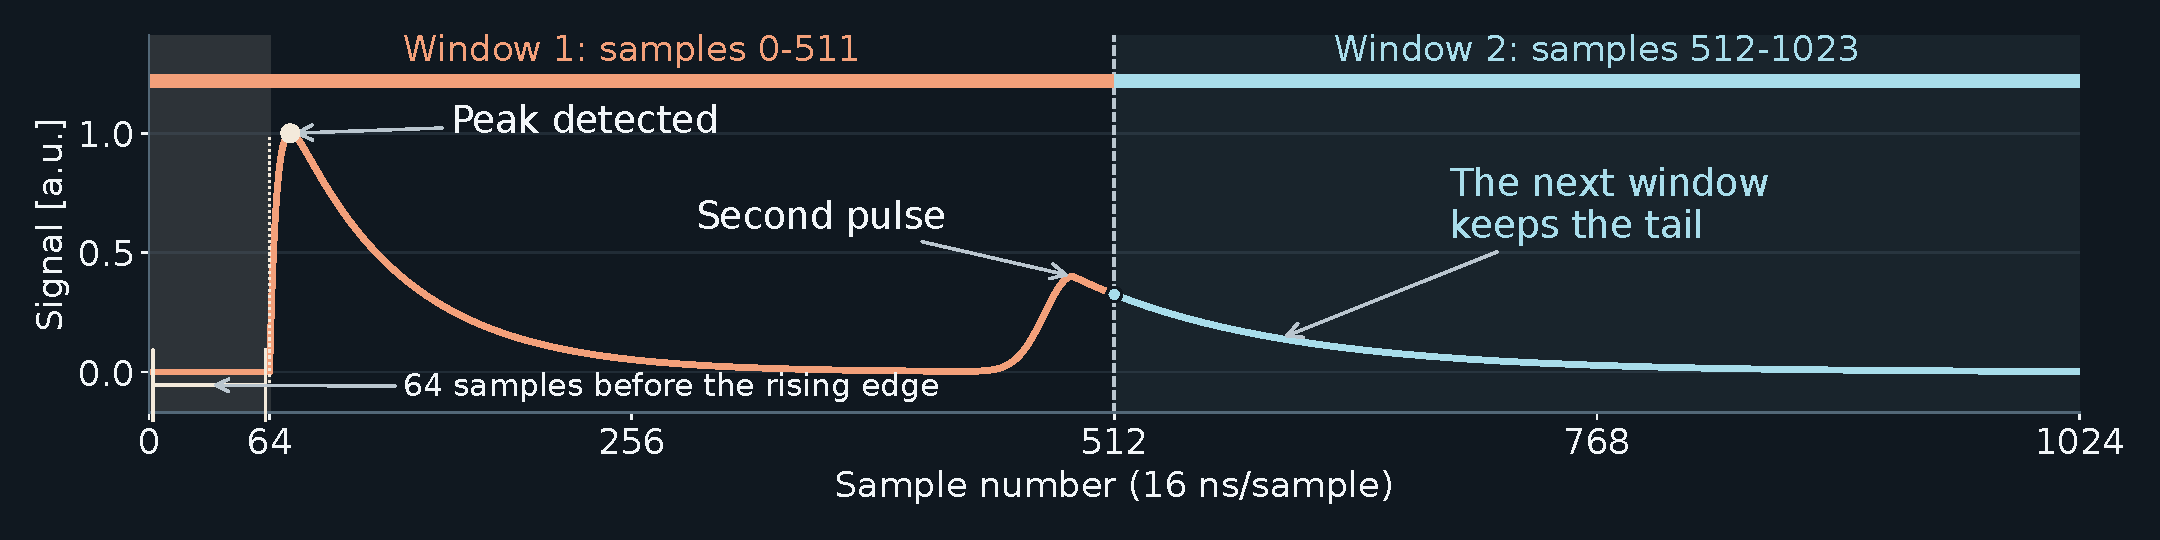
\includegraphics[width=\textwidth,height=0.54\textheight,keepaspectratio]{figures/pulse-windows.pdf}\par
  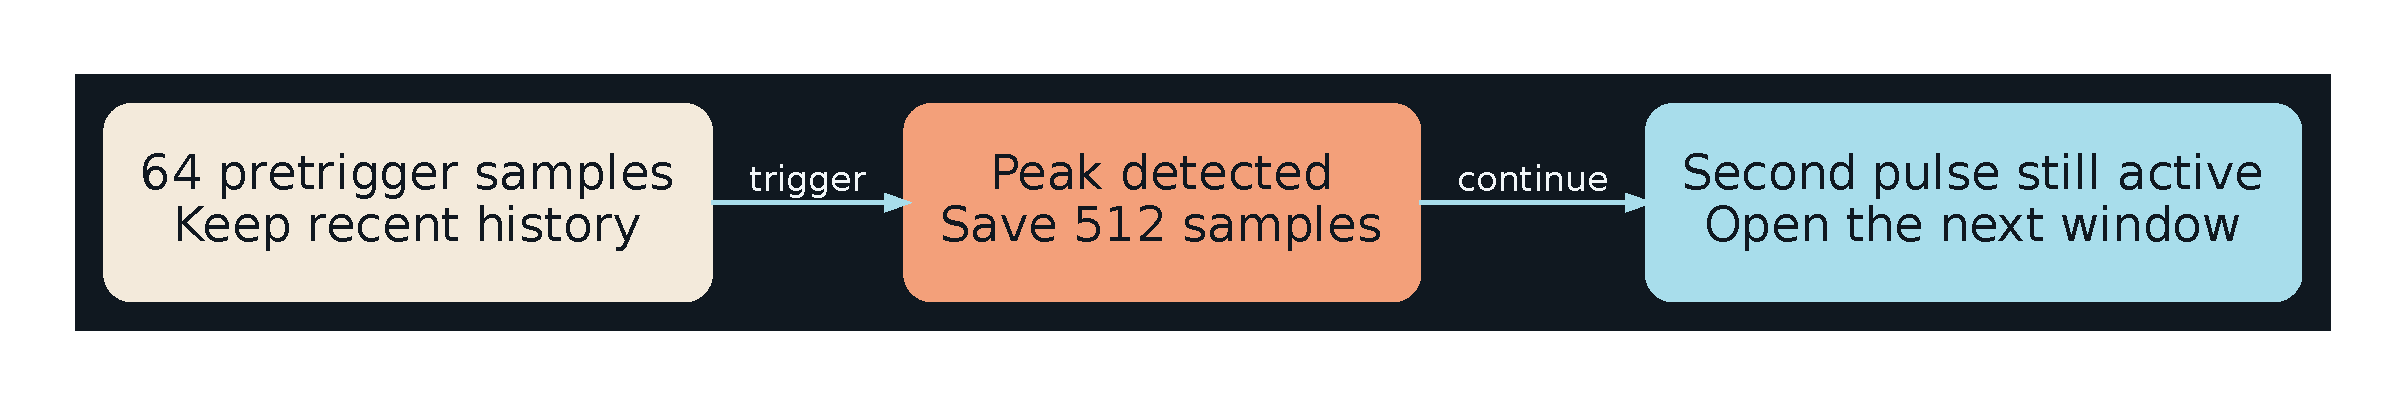
\includegraphics[width=0.94\textwidth,height=0.24\textheight,keepaspectratio]{diagrams/windows.pdf}\par
  \DuneDiagramCaption{Illustration: the boundary splits the record, while continuation keeps the second pulse's tail.}
\end{frame}

\begin{frame}{The milestone is agreement with full stream}
  \DuneBigStatement{THE GOAL}{Keep the same signal.\\ Make it easier to trigger on.}
    {Match signal timing and charge, while giving the DAQ peak descriptors for online coincidences.}
\end{frame}

\begin{frame}{Full stream leaves pulse finding to the DAQ}
  \centering
  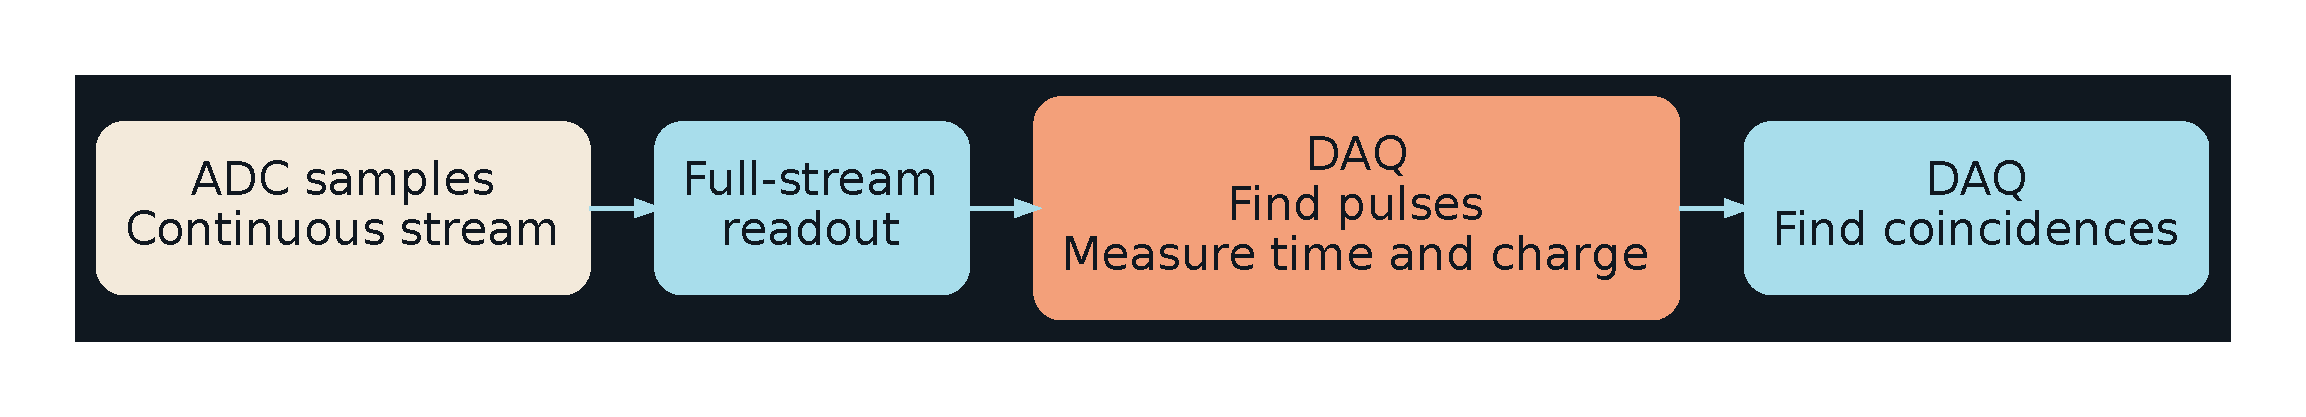
\includegraphics[width=\textwidth,height=0.64\textheight,keepaspectratio]{diagrams/raw-processing.pdf}\par
  \DuneDiagramCaption{Raw waveforms still need online pulse finding before the DAQ can compare photon times.}
\end{frame}

\begin{frame}{Raw streaming is a computing problem}
  \DuneBigStatement{32 CHANNELS AT 62.5 MS/s}{Two billion samples every second.}
    {The DAQ must find pulses in that stream.\\ FPGA peak descriptors let the online trigger start from pulse information.}
  {Per-board sample workload. \\Local FD documents separate photon readout and trigger processing; they do not give a measured PDS pulse-finding limit. \\ We have an storage limit with computing group.}
\end{frame}


\begin{frame}{Self-trigger moves that work into the FPGA}
  \centering
  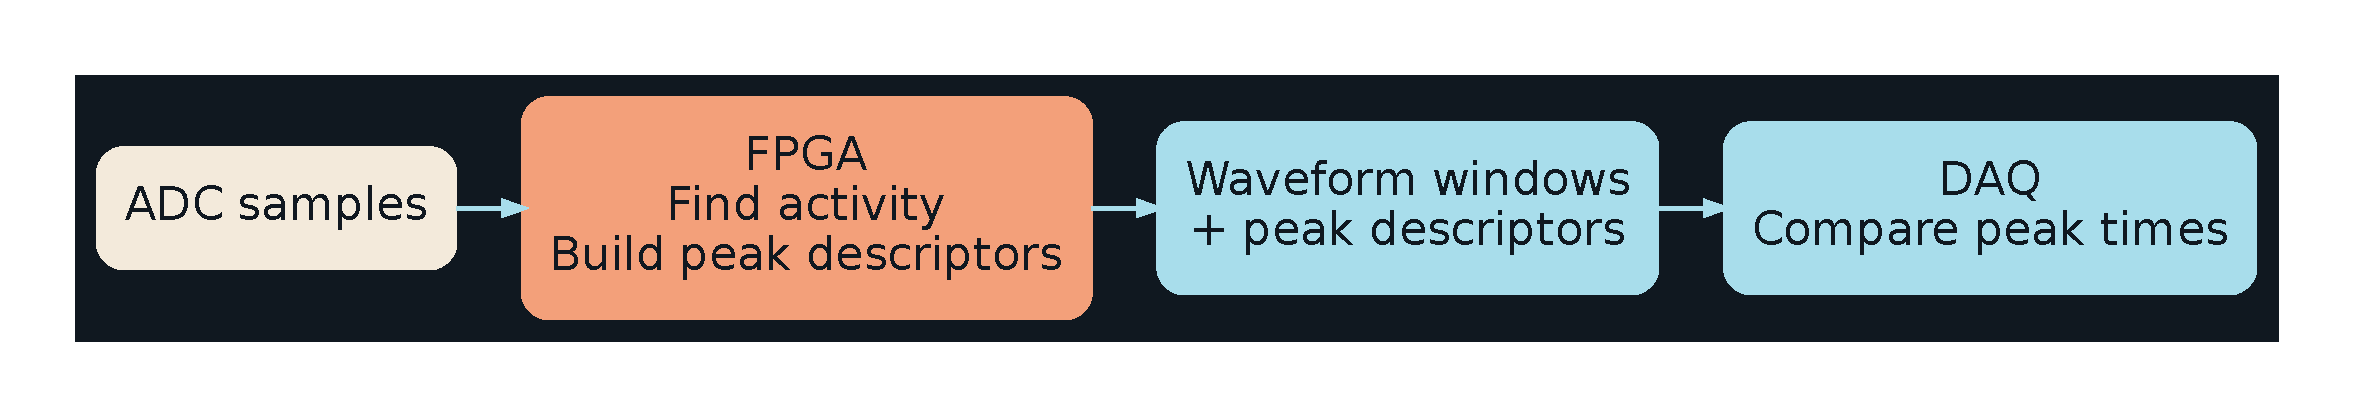
\includegraphics[width=\textwidth,height=0.64\textheight,keepaspectratio]{diagrams/preprocessing.pdf}\par
  \DuneDiagramCaption{Peak descriptors travel with the waveform.\\ The DAQ can use their times without repeating pulse finding on every sample.}
\end{frame}

\begin{frame}{Coincidences can form local PDS trigger activity}
  \centering
  \begin{tikzpicture}[x=1cm,y=1cm]
    \fill[DuneSky!15!DuneBackground] (4.2,0.3) rectangle (5.2,3.3);
    \foreach \y/\label in {3/A,2/B,1/C} {
      \node[text=DuneText,anchor=east] at (0.9,\y) {Channel \label};
      \draw[DuneTextMuted,line width=0.8pt] (1.2,\y) -- (8.3,\y);
    }
    \foreach \x/\y in {2/3,4.5/3,4.8/2,4.6/1,7.3/1} {
      \fill[DuneEditorialAccent] (\x,\y) circle (0.09);
    }
    \node[text=DuneSky,anchor=south] at (4.7,3.5) {Same time window};
    \draw[-Latex,DuneSky,line width=1.2pt] (5.3,2) -- (8.7,2);
    \node[fill=DuneEditorialAccent,text=DuneOnAccent,rounded corners,align=center,inner sep=10pt] at (10.2,2) {Local PDS\\trigger activity};
    \draw[-Latex,DuneTextMuted,line width=0.8pt] (1.2,0.15) -- (8.3,0.15);
    \node[text=DuneTextMuted,anchor=north] at (4.7,0.05) {Descriptor time};
  \end{tikzpicture}\par
  \DuneDiagramCaption{Illustration. Compare times across channels on a shared clock.\\ Tune the coincidence window and multiplicity using signal and background studies.}
\end{frame}

\begin{frame}{Four channels share one builder}
  \centering
  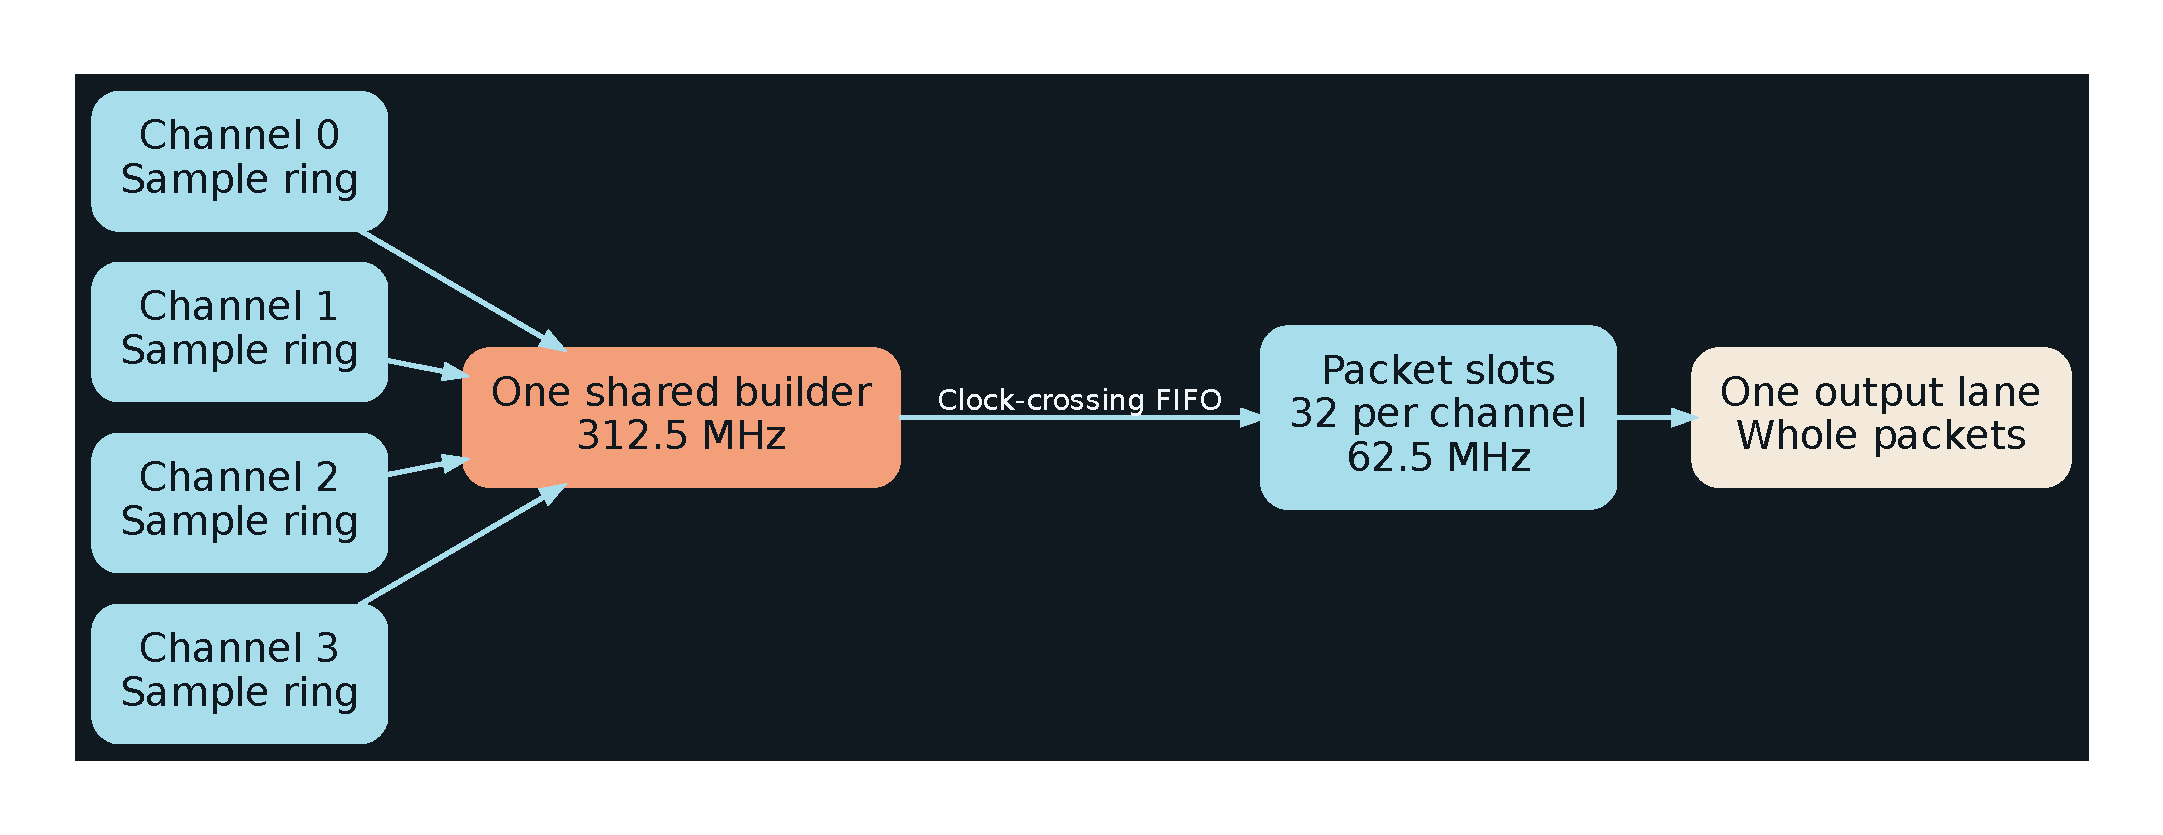
\includegraphics[width=\textwidth,height=0.64\textheight,keepaspectratio]{diagrams/architecture.pdf}\par
  \DuneDiagramCaption{Each builder packs waveform records and calculates peak descriptors. Eight builders serve 32 channels.}
\end{frame}

\begin{frame}{Replay the same signals through all three}
  \centering
  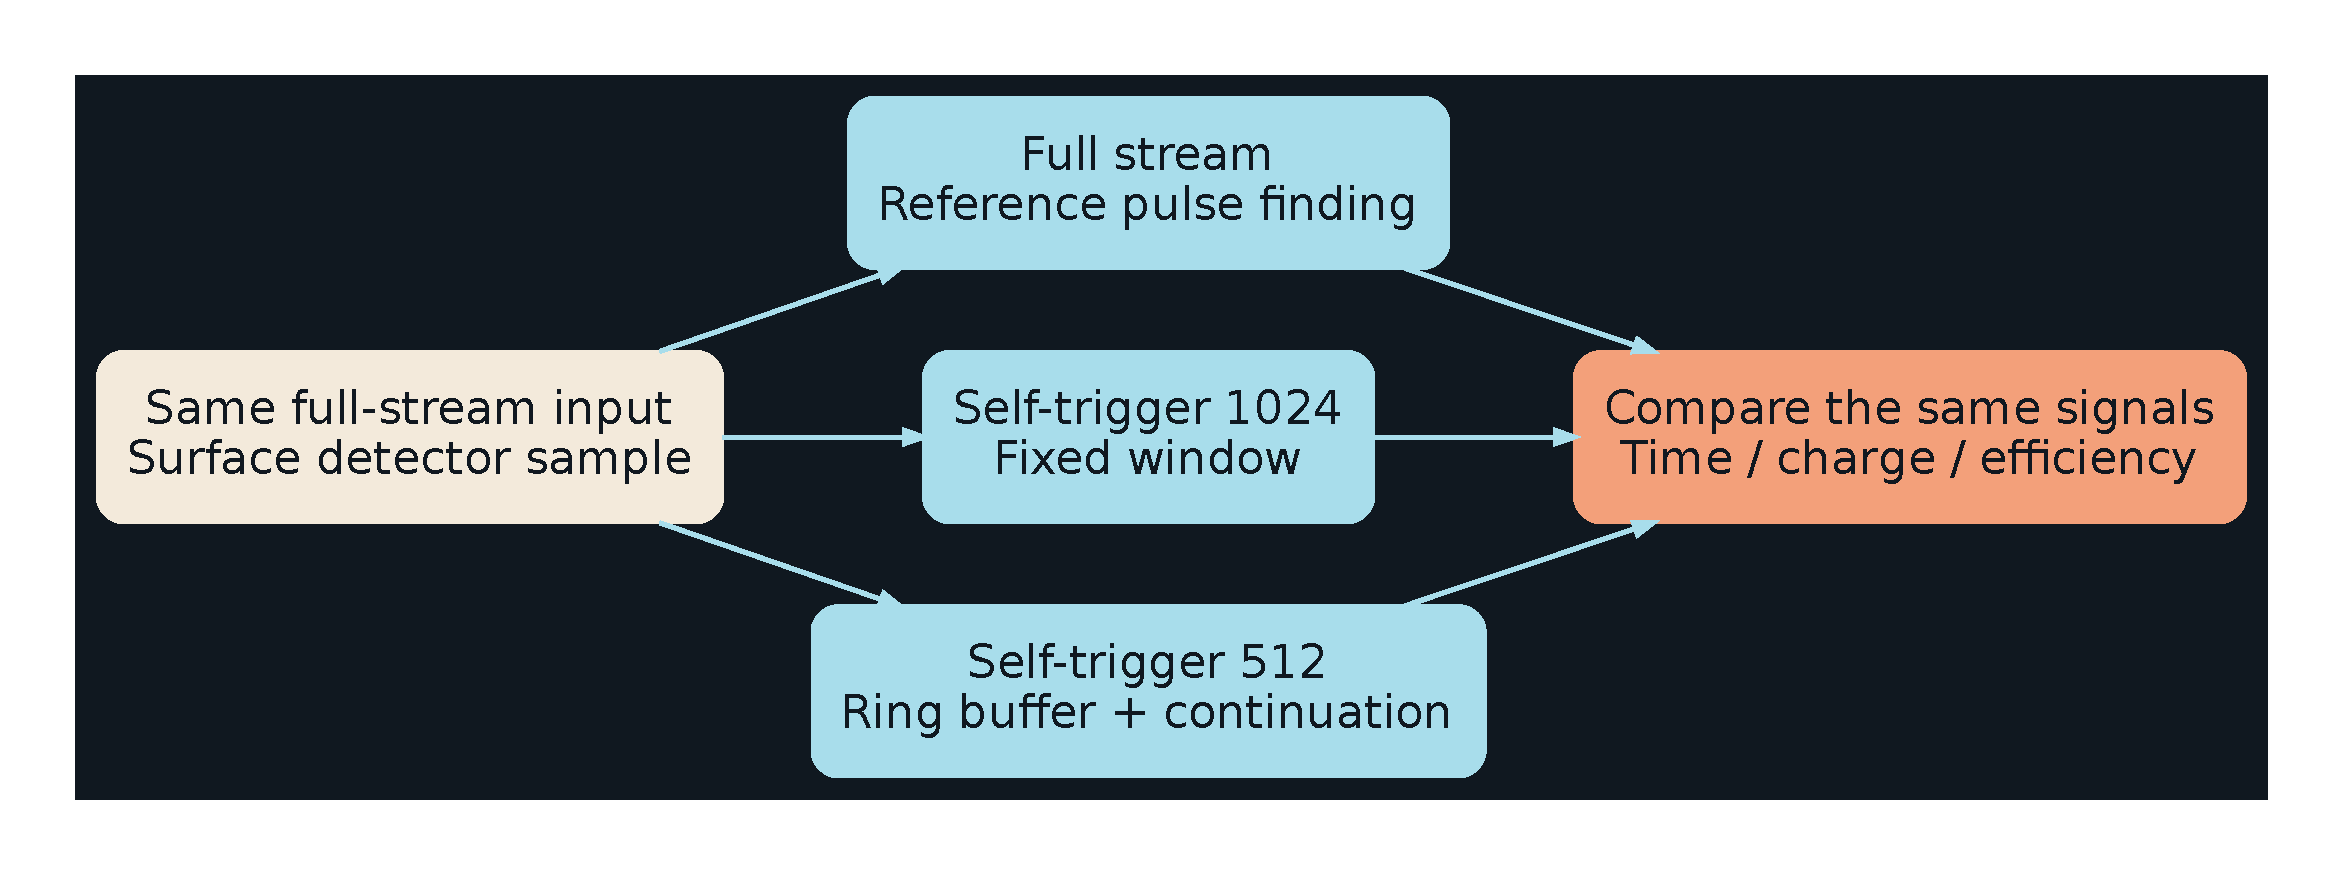
\includegraphics[width=\textwidth,height=0.64\textheight,keepaspectratio]{diagrams/milestone.pdf}\par
  \DuneDiagramCaption{Use the same surface full-stream input, thresholds, and output limits.\\ Compare recovered pulses, peak times, and charge. Matched three-way results are still needed.}
\end{frame}

\begin{frame}{The peak descriptors match the input waveform}
  \DuneBigStatement{FRESH RTL REPLAY}{379,656 descriptor words checked.}
    {An independent calculation checks each saved record's peak summaries against the known input.}
  \DuneDiagramCaption{Five deterministic cases. This checks descriptor correctness; it does not yet test local coincidence activity.}
\end{frame}


\begin{frame}{Saving samples is not the same as finding pulses}
  \centering
  \renewcommand{\arraystretch}{1.6}
  \begin{tabular}{@{}lll@{}}
    \toprule
    Readout & Sample retention & Pulse finding \\
    \midrule
    Self-trigger 1024 & Limited by busy windows & FPGA descriptors \\
    Self-trigger 512 + ring & Buffers reduce losses & FPGA descriptors \\
    Full stream & Every sample$^{*}$ & DAQ must find the peaks \\
    \bottomrule
  \end{tabular}\par\medskip
  Full stream is the sample reference.\par\smallskip
  Self-trigger moves pulse finding into the FPGA.\par\medskip
  \DuneDiagramCaption{$^{*}$Assuming lossless transport and storage. Saving all samples does not guarantee finding every pulse online.}
\end{frame}

\begin{frame}{More peak slots cost readout capacity}
  \centering
  {\small
  \renewcommand{\arraystretch}{1.18}
  \begin{tabular}{@{}lrrr@{}}
    \toprule
    Samples / peak slots & Bytes / frame & Missing descriptors & Dense lane use \\
    \midrule
    Current 512 / 5 & 960 & 50.3\% & 95.31\% \\
    Compact 512 / 5 & 952 & 50.3\% & 94.53\% \\
    256 / 2 & 480 & 61.3\% & 96.88\% \\
    256 / 3 & 488 & 44.9\% & 98.44\% \\
    256 / 5 & 504 & 18.9\% & \textcolor{DuneEditorialAccent}{101.56\%} \\
    \bottomrule
  \end{tabular}\par}
  \vspace{0.04cm}
  {\small
  \(\displaystyle
    U_{\mathrm{lane}}=\frac{4\,(B/8+2)}{N}\times100\%
    \qquad
    U_{256/5}=\frac{4\,(63+2)}{256}\times100\%=101.56\%
  \)\par\smallskip
  \(B\): frame bytes; \(N\): samples. Four channels share one internal lane.\par
  One 64-bit word per cycle, plus two cycles per frame; continuous capture.\par
  Above 100\%: sustained backlog. Intermittent capture uses less capacity.\par}
  \vspace{0.04cm}
  \DuneDiagramCaption{Descriptor loss: one synthetic case, 40 detected photons/channel/burst, 1.6\,\(\mu\)s slow light, extrapolated +5 V afterpulsing. Simplified peak-count model; waveform charge retained.}
\end{frame}


\begin{frame}{LArSoft supplies the detector-side load}
  \centering
  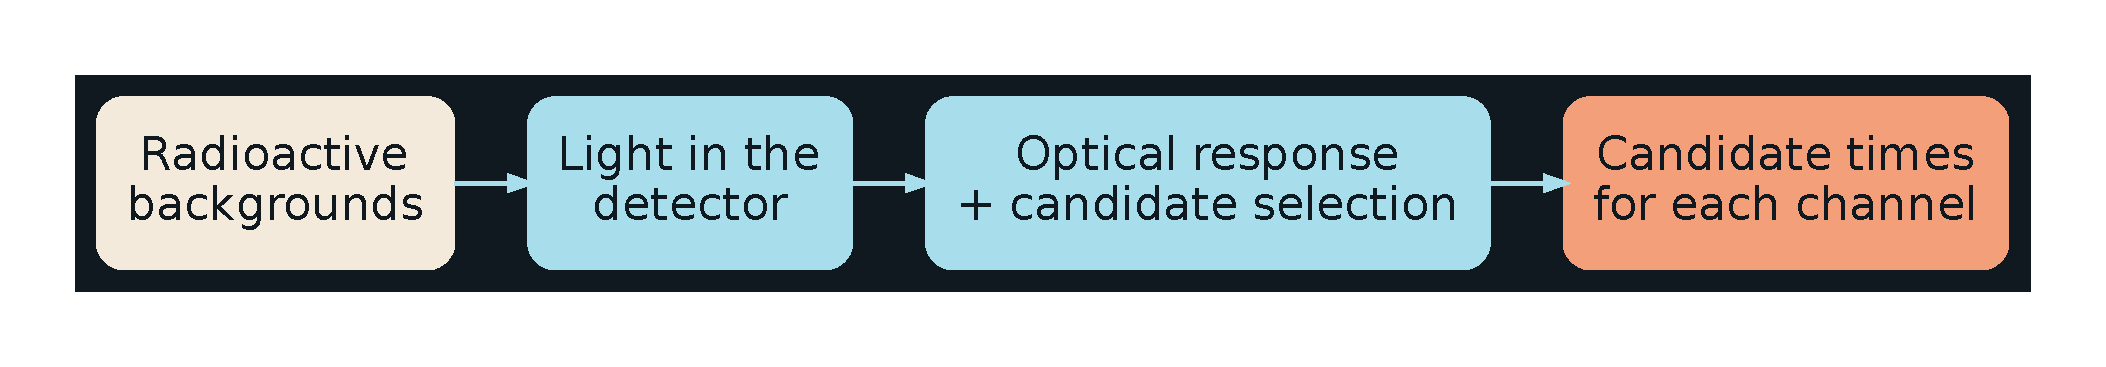
\includegraphics[width=\textwidth,height=0.64\textheight,keepaspectratio]{diagrams/larsoft.pdf}\par
  \DuneDiagramCaption{Use physical activity to test pulse finding and coincidences. The grouped RTL replay currently uses synthetic waveforms.}
\end{frame}

\begin{frame}{The VD cathode sees the most activity}
  \centering
  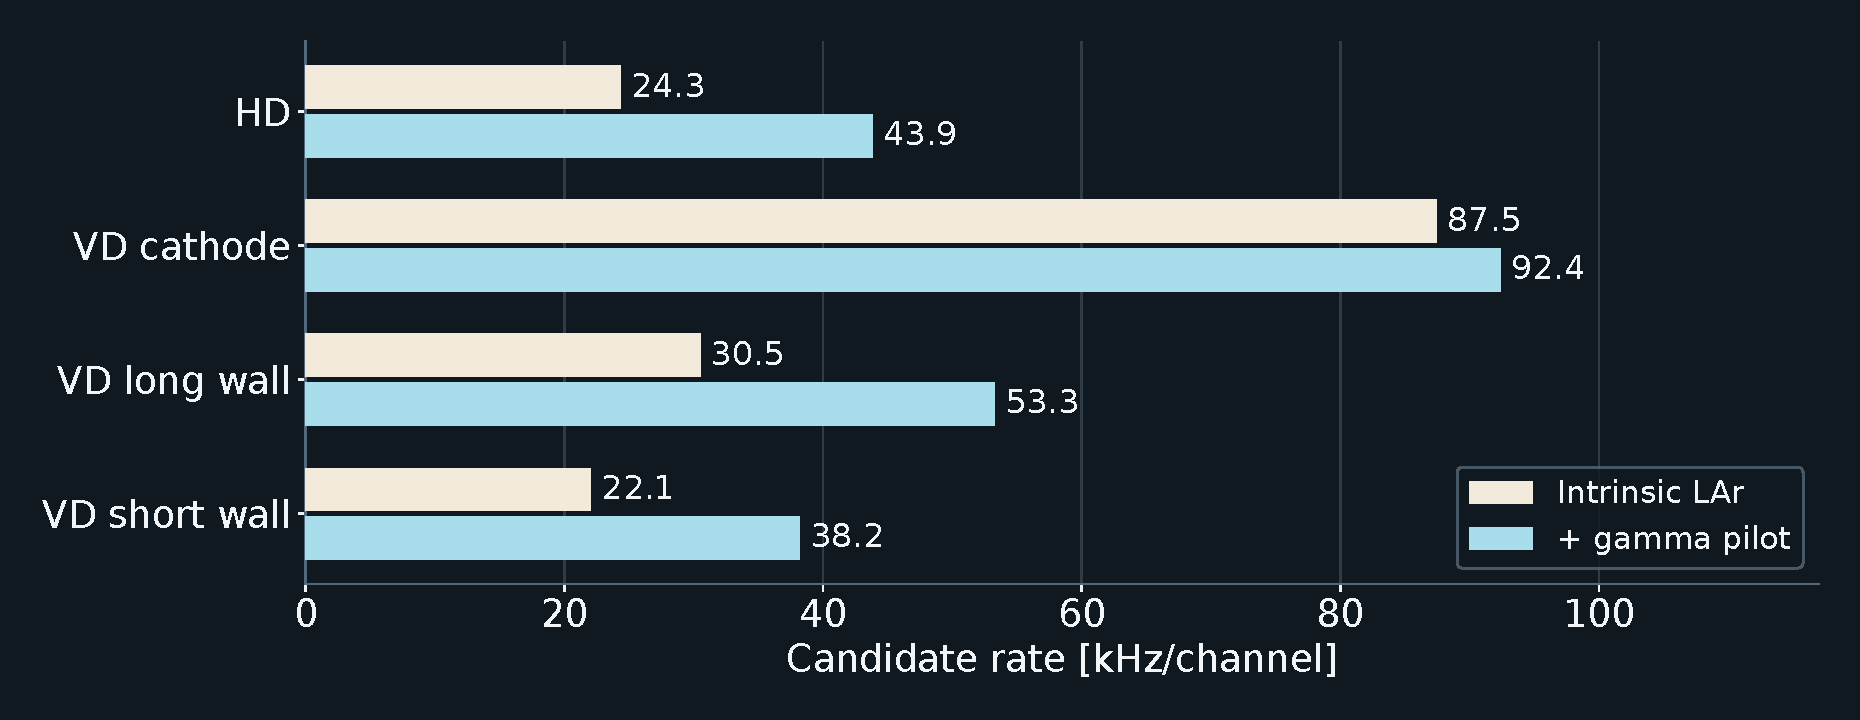
\includegraphics[width=\textwidth,height=0.68\textheight,keepaspectratio]{figures/larsoft-rates.pdf}\par
  \DuneDiagramCaption{Mean candidate rates above 0.7 PE. Intrinsic LAr: eight shards. Gamma addition: one window per source family, still a pilot.}
\end{frame}

\begin{frame}{Show the same signals in both readouts}
  \centering
  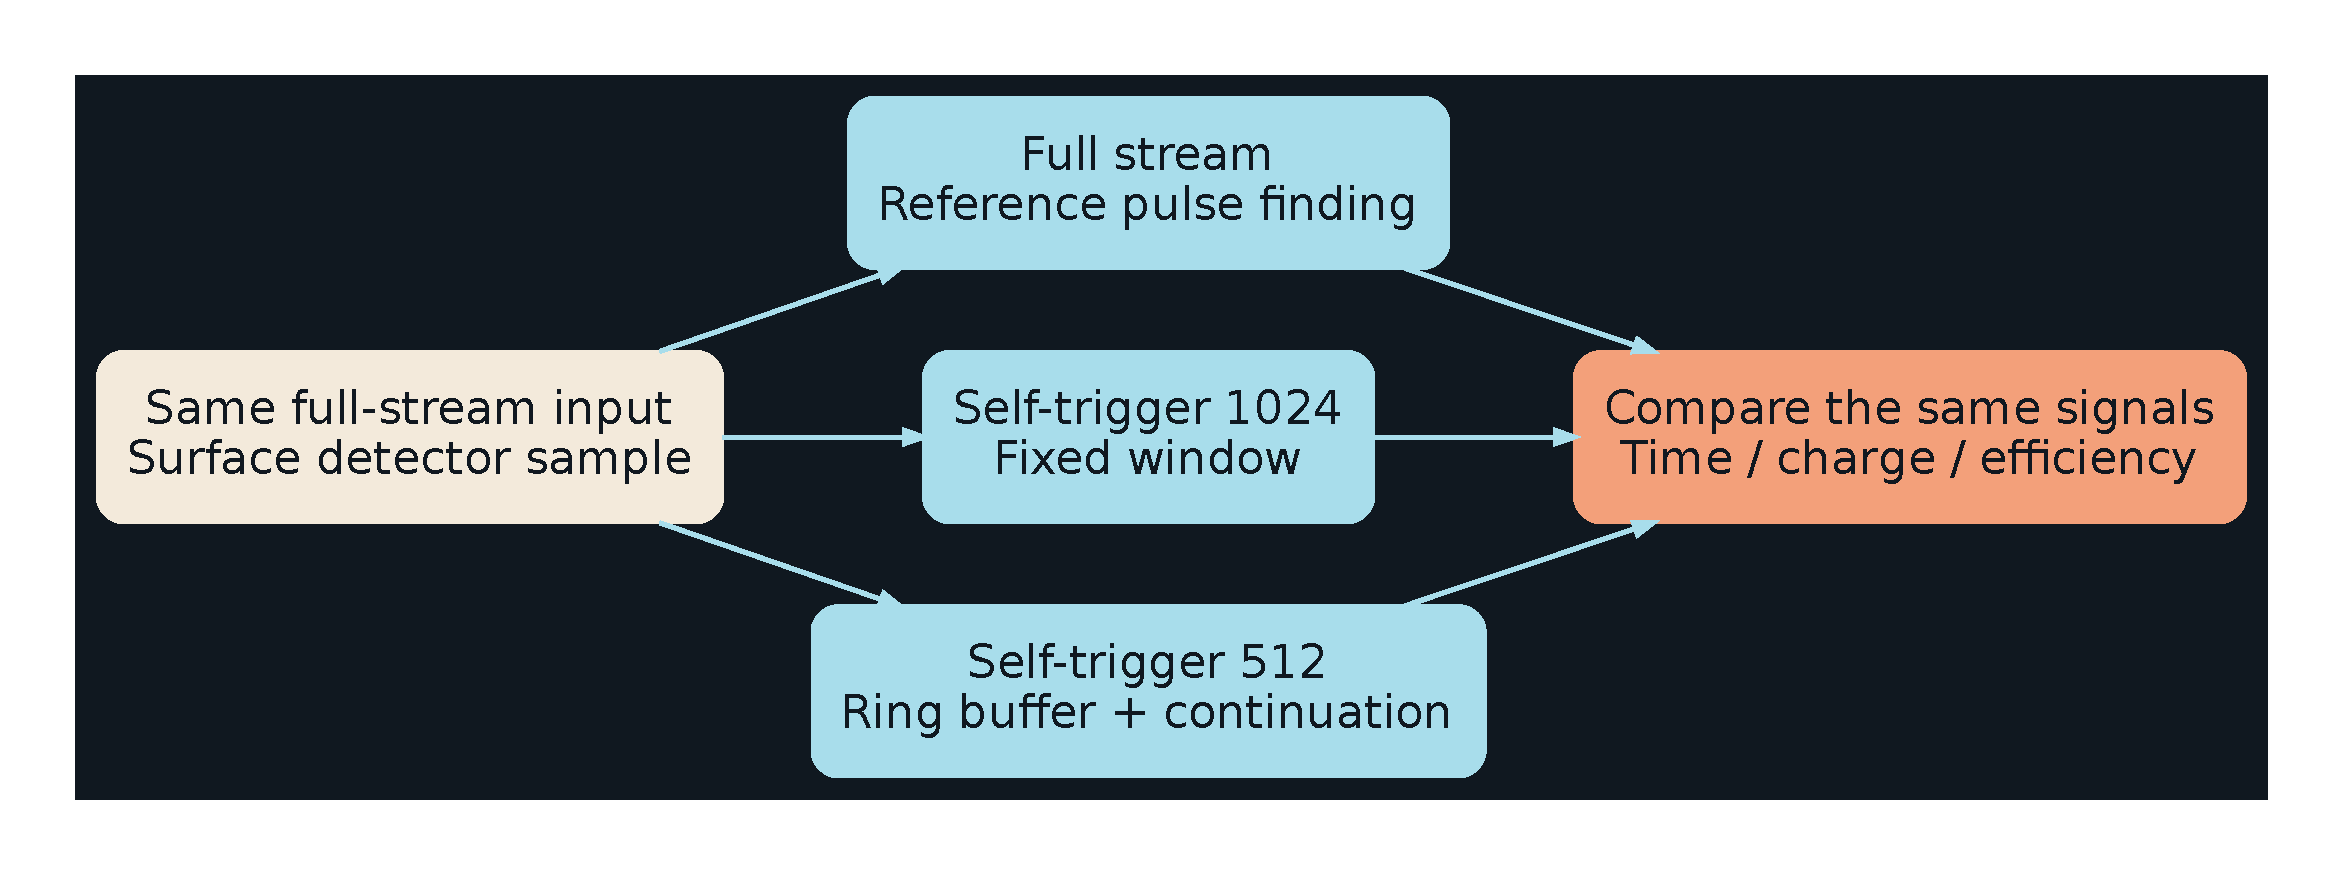
\includegraphics[width=\textwidth,height=0.64\textheight,keepaspectratio]{diagrams/milestone.pdf}\par
  \DuneDiagramCaption{The milestone test: matched waveforms and backgrounds, then matched signal timing, charge, and local trigger activity.}
\end{frame}

\appendix
\DuneSectionPage{BACKUP}{Why this helps}
  {Dead time and low-energy physics without a beam gate.}

\begin{frame}{Buffers buy time}
  \DuneBigStatement{SHORT STALLS}{Keep collecting while the output waits.}
    {The ring holds recent samples. Reserved packet slots hold complete records. Long stalls eventually fill both.}
\end{frame}

\begin{frame}{Continuation keeps the tail}
  \DuneBigStatement{LONG PULSES}{Add another 512 samples when needed.}
    {Short pulses stay short. Sustained activity can span adjacent records. Check recovered charge to see whether the tail survives.}
\end{frame}

\begin{frame}{We cannot wait for the beam}
  \DuneBigStatement{LOW-ENERGY PHYSICS}{Keep the light from weak signals.}
    {Preserving low-energy light signals can support background rejection and searches for solar and supernova neutrinos.}
  \DuneDiagramCaption{Study question: can better background tagging let us use more of the detector?}
  \DuneSourceLine{DUNE Phase II: low-energy physics opportunities}{https://cds.cern.ch/record/2909101/files/document.pdf}
\end{frame}

\begin{frame}{Start with the surface full-stream data}
  \DuneBigStatement{A PESSIMISTIC STRESS TEST}{We already have a demanding sample in xc\_sim.}
    {Replay it through self-trigger. Compare the saved waveform, peak times, and charge against the raw data.}
  \DuneDiagramCaption{Surface-detector activity tests robustness under a harsh load. It does not set the underground far-detector background rate.}
\end{frame}

\begin{frame}{Each pulse gets a start, height, area, and duration}
  \centering
  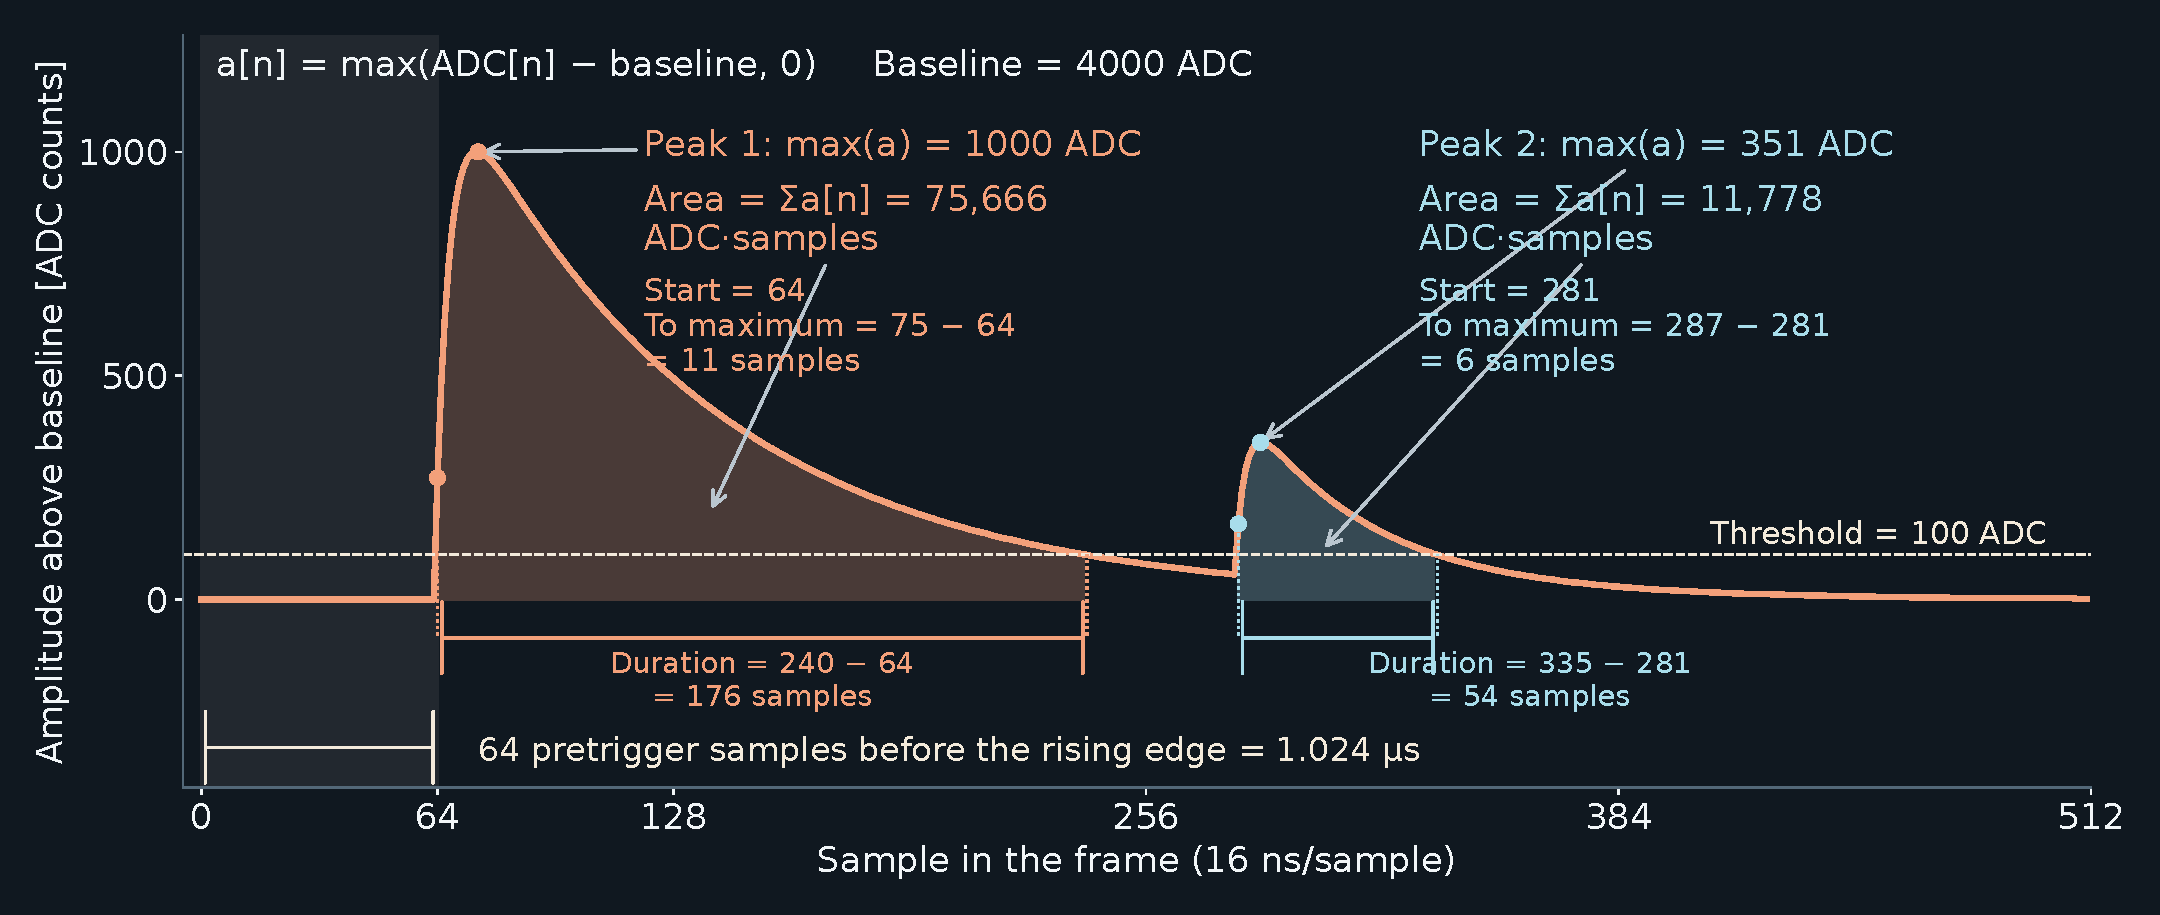
\includegraphics[width=\textwidth,height=0.70\textheight,keepaspectratio]{figures/descriptor-time.pdf}\par
  \DuneDiagramCaption{Sum amplitudes above threshold; do not subtract the threshold. Both slots valid; format byte 0xF1. Illustrative waveform.}
\end{frame}

\begin{frame}{Five peak descriptors now cover half the waveform}
  \centering
  \begin{tikzpicture}[x=1cm,y=1cm]
    \node[text=DuneText,anchor=east] at (0.0,2.6) {1024 samples};
    \node[text=DuneText,anchor=east] at (0.0,0.9) {512 samples};
    \draw[DunePaper,line width=1.2pt] (0.3,2.1) rectangle (10.3,3.1);
    \node[text=DunePaper] at (5.3,2.6) {One waveform: up to 5 peak descriptors};
    \draw[DuneEditorialAccent,line width=1.5pt] (0.3,0.4) rectangle (5.3,1.4);
    \draw[DuneSky,line width=1.5pt] (5.3,0.4) rectangle (10.3,1.4);
    \node[text=DuneEditorialAccent,align=center] at (2.8,0.9) {First 512 samples\\up to 5 descriptors};
    \node[text=DuneSky,align=center] at (7.8,0.9) {Next 512 samples\\up to 5 descriptors};
    \foreach \x/\label in {0.3/0,5.3/512,10.3/1024} {
      \node[text=DuneTextMuted,anchor=north] at (\x,0.15) {\label};
    }
  \end{tikzpicture}\par
  \DuneDiagramCaption{The same five-peak format gives finer descriptor coverage: up to ten peak summaries over 1024 samples when both fragments are retained.}
\end{frame}

% Generated by render_results.py; edit the generator, not this file.
\begin{frame}{Every common packet matches}
  \framesubtitle{Fresh five-mode RTL replay; firmware 7a25777e}
  \small
  \renewcommand{\arraystretch}{1.3}
  \begin{tabular}{@{}lrrrr@{}}
    \toprule
    Mode & Grouped packets & Native packets & Common / identical & Max latency [$\mu$s] \\
    \midrule
    0 & 3,392 & 3,392 & 3,392 & 17.984 \\
    1 & 3,372 & 3,372 & 3,372 & 17.952 \\
    2 & 2,224 & 2,200 & 2,200 & 560.432 \\
    3 & 3,672 & 3,446 & 944 & 48.272 \\
    4 & 3,296 & 3,272 & 3,272 & 17.984 \\
    \bottomrule
  \end{tabular}\par
  \medskip
  13,180 common packets are byte-identical; 16,198,656 ADC samples checked across both implementations.\par\medskip
  Mode 4 includes deliberate reset and disable losses. Latency runs from the first sample to the final output word.
\end{frame}


\begin{frame}{Count saved samples, not just packets}
  \centering
  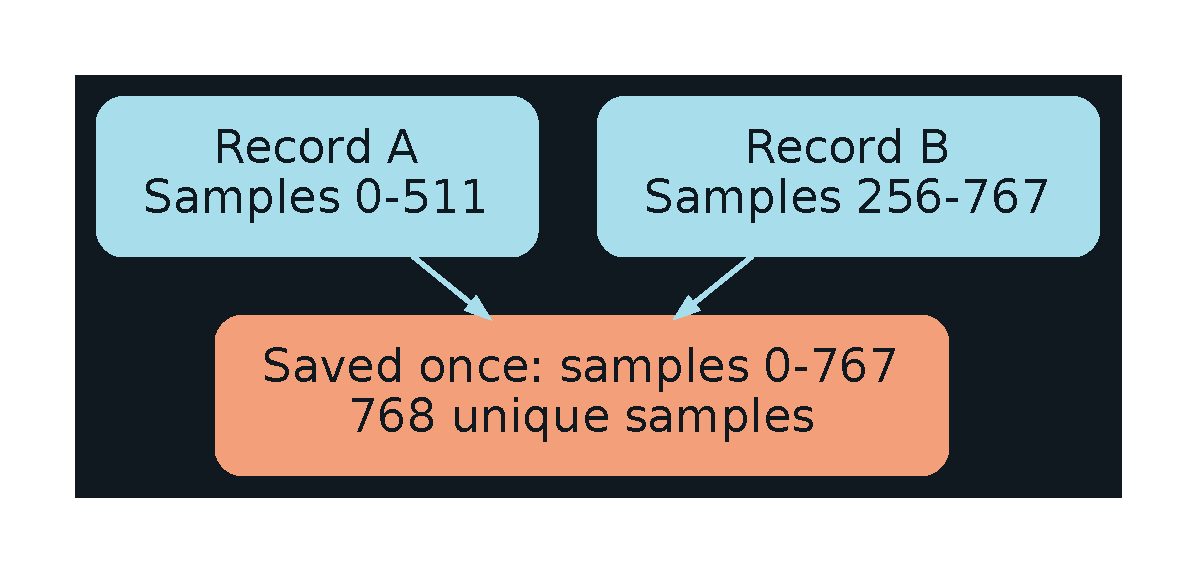
\includegraphics[width=0.91\textwidth,height=0.62\textheight,keepaspectratio]{diagrams/coverage.pdf}\par
  \DuneDiagramCaption{Merge overlapping windows before measuring loss. Each nonzero input sample counts once; quiet samples are outside the denominator.}
\end{frame}

\begin{frame}{Stop the output and watch what happens}
  \DuneBigStatement{ONE STRESS TEST}{Pause all lanes for 544 microseconds.}
    {Let the buffers fill. Restart readout. Check what was kept, what was lost, and whether it recovers.}
  \DuneDiagramCaption{Other cases check simultaneous pulses, short stalls, overlapping triggers, and reset.}
\end{frame}

\begin{frame}{Eight lanes feed four links}
  \centering
  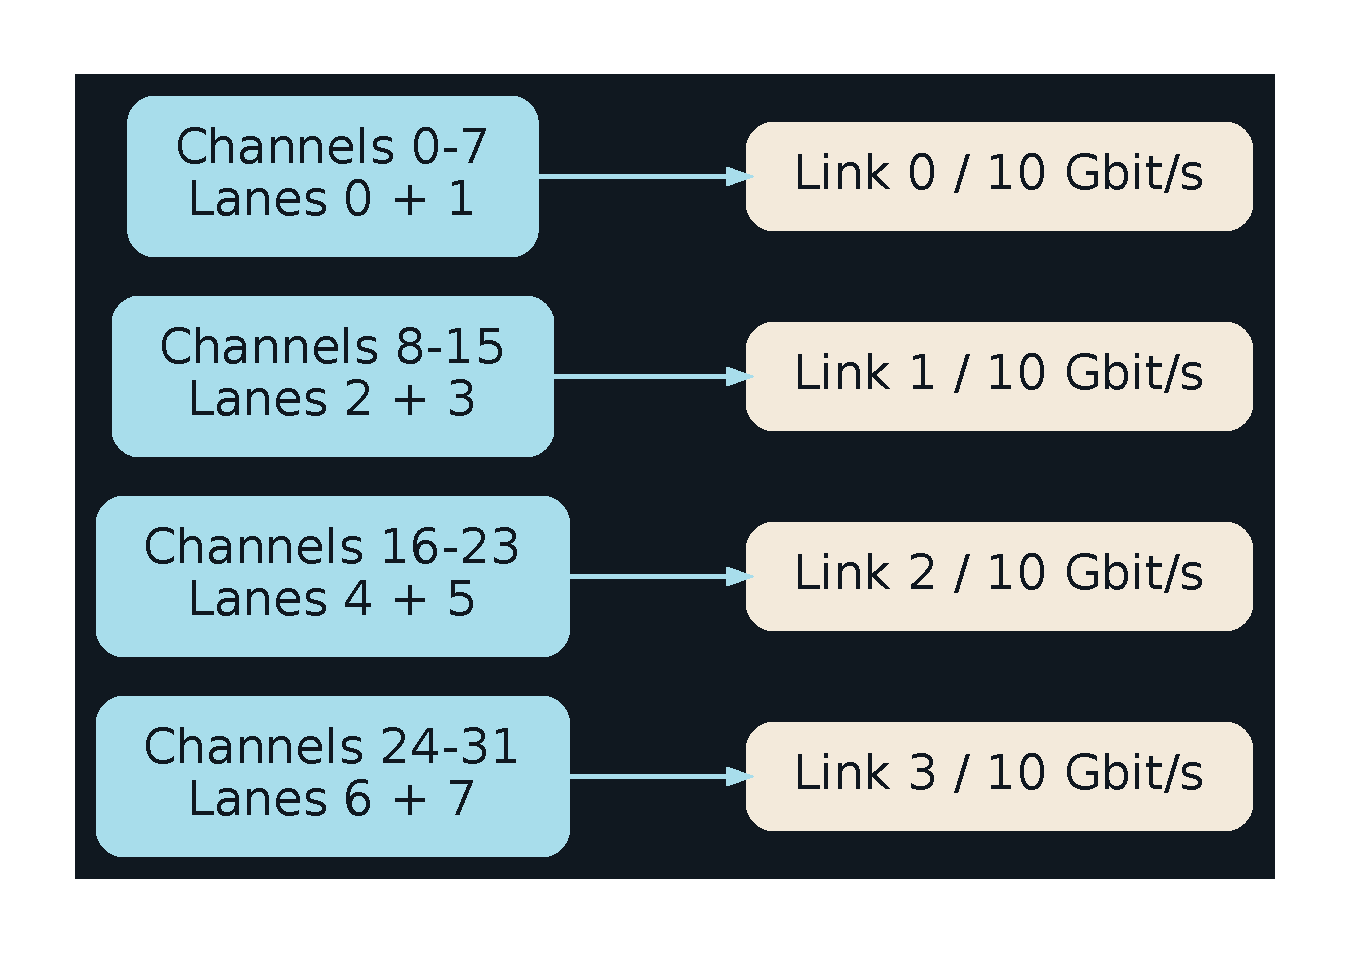
\includegraphics[width=0.90\textwidth,height=0.68\textheight,keepaspectratio]{diagrams/links.pdf}\par
  \DuneDiagramCaption{Grouped32 mapping. The replay checks the lanes; it does not send data through physical Ethernet.}
\end{frame}

\begin{frame}{Full stream also pairs two streams per link}
  \centering
  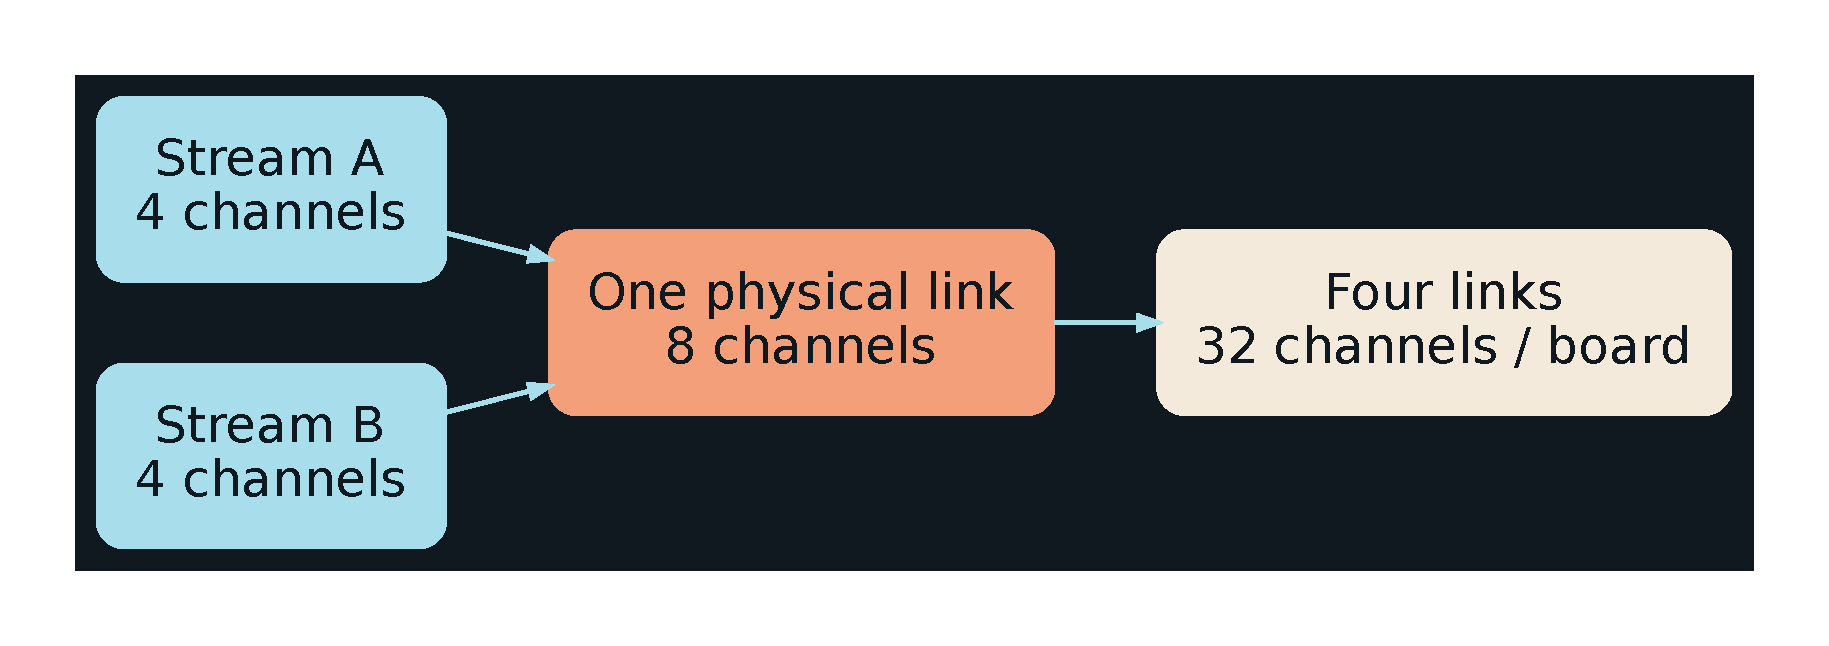
\includegraphics[width=\textwidth,height=0.64\textheight,keepaspectratio]{diagrams/fullstream-mapping.pdf}\par
  \DuneDiagramCaption{Checked full-stream source: four channels per logical stream, eight per physical link, 32 per board. Installed image and channel selection were not checked.}
\end{frame}

\begin{frame}{Expected traffic from the modeled activity only}
  \centering
  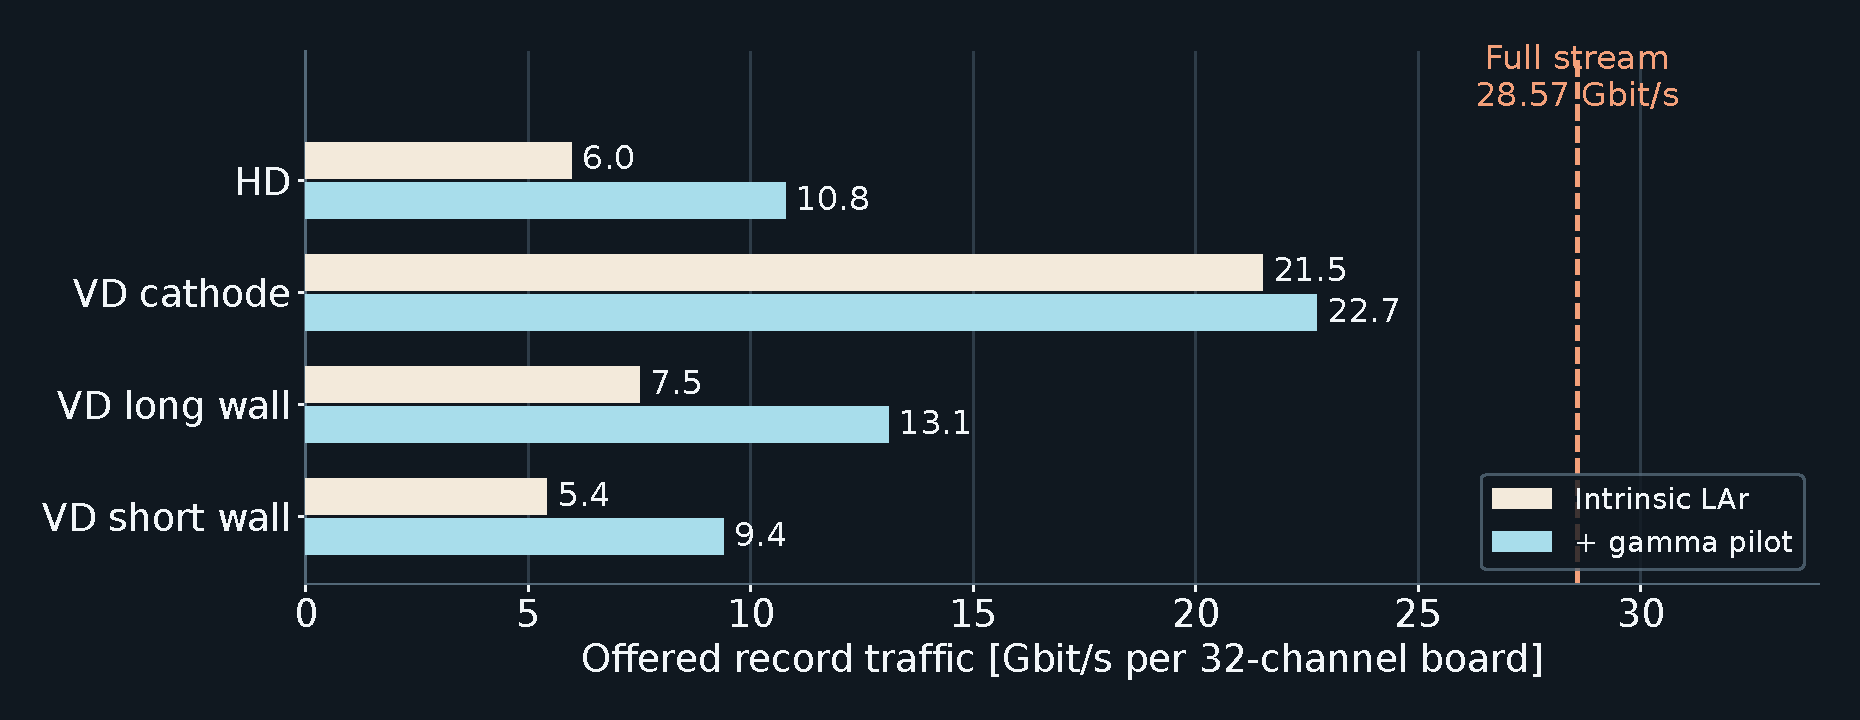
\includegraphics[width=\textwidth,height=0.68\textheight,keepaspectratio]{figures/traffic.pdf}\par
  \DuneDiagramCaption{Other background sources are not included. 32 channels; one self-trigger record per candidate, before losses or continuation. Both estimates exclude network overhead.}
\end{frame}

\begin{frame}{Full stream is constant; self-trigger follows activity}
  \centering
  \renewcommand{\arraystretch}{1.5}
  \begin{tabular}{@{}lll@{}}
    \toprule
    Same 32-channel board & Full stream & Self-trigger 512 + ring \\
    \midrule
    What is sent? & Every sample & Selected windows + peaks \\
    What sets the rate? & ADC sample clock & Saved records per second \\
    HD example below & 28.57 Gbit/s & 10.78 Gbit/s \\
    \bottomrule
  \end{tabular}\par\medskip
  HD intrinsic + gamma pilot: 43,855 candidates/s/channel.\par\smallskip
  $32\times43{,}855\times960\ \mathrm{bytes}\times8
     =10.78\ \mathrm{Gbit/s}$.\par\medskip
  \DuneDiagramCaption{Estimate: one 512-sample record per candidate; no continuation, merging, or losses modeled. Other backgrounds are excluded. Both rates include record headers, not network overhead.}
\end{frame}

\begin{frame}{Preprocessing matters even when traffic stays high}
  \DuneBigStatement{CONTINUOUS ACTIVITY}{The descriptors still save pulse-finding work.}
    {Continuous self-trigger records reach 30 Gbit/s for 32 channels. Bandwidth savings can disappear while the preprocessing benefit remains.}
\end{frame}

\begin{frame}{The LArSoft numbers are a dated snapshot}
  \small
  \begin{tabular}{@{}ll@{}}
  \toprule
  Software & dunesw v10\_22\_00d01; larsoft v10\_22\_00 \\
  Detector models & FD horizontal drift (HD), vertical drift (VD) \\
  Candidate selection & Above 0.7 photoelectrons (PE); no 10 MeV cut \\
  Intrinsic baseline & Atmospheric argon mixture; eight shards \\
  Gamma addition & One physical window per source family \\
  Snapshot & 9 September 2026; reused here, not rerun \\
  \bottomrule
  \end{tabular}\par\medskip
  Shared transport, a complete background inventory, and calibrated noise are still needed for a detector trigger prediction.
\end{frame}

\begin{frame}{Keep the result tied to its inputs}
  \small
  \textbf{Firmware:} \texttt{7a25777e}, grouped32 branch.\par\medskip
  \textbf{Run:} \texttt{scripts/run\_grouped32\_rtl\_study.py --run}.\par\medskip
  \textbf{Evidence:} this deck's README, JSON reports, CSV tables, and figure scripts.\par\medskip
  Behavioral memory and clock-crossing models; no physical Ethernet or analog capture test.
  \DuneSourceLine{Firmware architecture and verification}{\firmwaresource/docs/reports/grouped32/approval-review-20260915.md}
\end{frame}

\end{document}
